\documentclass[../../main.tex]{subfiles}
\begin{document}

\subsection*{2.1}
Una carica $q = 1.39 * 10^{-8}\ C$ è distribuita con densità superficiale uniforma $\sigma$ su una corona circolare piana di raggio interno $R_1 = 20\ cm$ e raggio esterno $R_2 = 30\ cm$.
\\a) Determinare le espressioni del campo elettrostatico $\vec{E(x)}$ e del poteniale $V(x)$ sull'asse della corona.
\\b) Calcolare l'energia cinetcia con la quale un elettrone libero in un punto P con $x_0 = 20\ cm$ raggiunge il centro.
\\c) Calcolare la forza agente su un dipolo elettrico di momento $p = p_0\vec{u_x}$ con $p_0 = 10^{-10}\ cm$, posto in O.
\\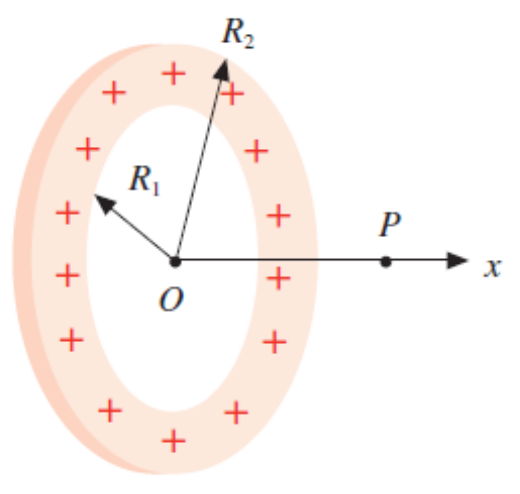
\includegraphics[scale=0.3]{e_2_1.png}
\subsubsection*{Formule utilizzate}

\subsubsection*{Soluzione punto a}
$\sigma = \frac{q}{\pi(R_2^2-R_1^2)} = \frac{1.39 * 10^{-8}}{3.14 * (0.3^2 - 0.2^2)} = 8.85 * 10^-8\ \frac{C}{m^2}$
\\$dq = \sigma ds = \sigma 2\pi rdr$
\\$dV = \frac{dq}{4\pi\epsilon_0\sqrt{r^2 + x^2}} = \frac{\sigma 2 \pi rdr}{4\pi\epsilon_0\sqrt{r^2+x^2}}$
\\$V = \frac{\sigma}{2\epsilon_0}\left[\sqrt{R_2^2 + x^2} - \sqrt{R_1^2 + x^2}\right]$
\\$E_x = -\frac{\delta V}{\delta x} = -\frac{\sigma}{2\epsilon_0}\left[\frac{x}{\sqrt{R_2^2 + x^2}} -\frac{x}{\sqrt{R_1^2+x^2}}\right]$
\subsubsection*{Soluzione punto b}
$\Delta E_k + \Delta U = 0$
\\$E_{k_{fin}} = E_{k_{in}} - e[V_{in} - V_{fin}] = -\frac{e\sigma}{2\epsilon_0}\left[\sqrt{R_2^2 + x_0^2}-\sqrt{R_1^2 + x_0^2}-R_2 + R_1\right] =111\ eV$
\subsubsection*{Soluzione punto c}
$\vec{F}\left(\vec{p}*\nabla\right)\vec{E} = p_0\left(\vec{u_x} * \nabla \right)\vec{E} = p_0 \frac{\delta \vec{E}}{\delta x}\vec{u_x}$
\\$E_x = -\frac{\sigma}{2\epsilon_0}\left[\frac{x}{\sqrt{R_2^2 + x^2}}-\frac{x}{\sqrt{R_1^2 +x^2}}\right]$
\\$\frac{\delta E_x}{\delta x} = -\frac{\sigma}{2\epsilon_0}\left[\frac{1}{\sqrt{R_2^2 + x^2}} - \frac{x^2}{(R_2^2 + x^2)^{\frac{3}{2}}}-\frac{1}{\sqrt{R_1^2 + x^2}} + \frac{x^2}{(R_1^2 + x^2)^{\frac{3}{2}}}\right]$
\\$F = \frac{p_0 \sigma}{2\epsilon_0}\left[\frac{1}{R_1}-\frac{1}{R_2}\right] = 8.33*10^{-7}\ N$
\newpage

\end{document}